%%% LaTeX Template: Two column article
%%%
%%% Source: http://www.howtotex.com/
%%% Feel free to distribute this template, but please keep to referal to http://www.howtotex.com/ here.
%%% Date: February 2011

%%% Preamble
\documentclass[	DIV=calc,%
							paper=a4,%
							fontsize=12pt,%
							onecolumn]{scrartcl}	 					% KOMA-article class

\usepackage{lipsum}													% Package to create dummy text
\usepackage[brazil]{babel}										% English language/hyphenation
\usepackage[protrusion=true,expansion=true]{microtype}				% Better typography
\usepackage{amsmath,amsfonts,amsthm}					% Math packages
\usepackage[pdftex]{graphicx}									% Enable pdflatex
\usepackage[svgnames]{xcolor}									% Enabling colors by their 'svgnames'
\usepackage[hang, small,labelfont=bf,up,textfont=it,up]{caption}	% Custom captions under/above floats
\usepackage{epstopdf}												% Converts .eps to .pdf
\usepackage{subfig}													% Subfigures
\usepackage{booktabs}
			% Nicer tables
\usepackage{float}
												
\usepackage{fix-cm}													% Custom fontsizes
\usepackage[utf8]{inputenc}
\usepackage[top=2.5cm, bottom=2.5cm, left=2.5cm, right=2.5cm]{geometry}
\usepackage[ddmmyyyy]{datetime}
\addto\captionsenglish{%
	\renewcommand\tablename{Tabela}
	\renewcommand\figurename{Figura}
} 
 

 
%%% Custom sectioning (sectsty package)
\usepackage{sectsty}													% Custom sectioning (see below)
\allsectionsfont{%															% Change font of al section commands
	\usefont{OT1}{phv}{b}{n}%										% bch-b-n: CharterBT-Bold font
	}

\sectionfont{%																% Change font of \section command
	\usefont{OT1}{phv}{b}{n}%										% bch-b-n: CharterBT-Bold font
	}



%%% Headers and footers
\usepackage{fancyhdr}												% Needed to define custom headers/footers
	\pagestyle{fancy}														% Enabling the custom headers/footers
\usepackage{lastpage}	

% Header (empty)
\lhead{}
\chead{}
\rhead{}
% Footer (you may change this to your own needs)

%% ====================================
%% ====================================
%% mude o rodape  do projeto
%% ====================================
%% ====================================

\lfoot{\footnotesize \texttt{Cabeamento estruturado} \textbullet ~Projeto}


\cfoot{}
\rfoot{\footnotesize Página \thepage\ de \pageref{LastPage}}	% "Page 1 of 2"
\renewcommand{\headrulewidth}{0.0pt}
\renewcommand{\footrulewidth}{0.4pt}



%%% Creating an initial of the very first character of the content
\usepackage{lettrine}
\newcommand{\initial}[1]{%
     \lettrine[lines=3,lhang=0.3,nindent=0em]{
     				\color{DarkBlue}
     				{\textsf{#1}}}{}}



%%% Title, author and date metadata
\usepackage{titling}															% For custom titles

\newcommand{\HorRule}{\color{DarkBlue}%			% Creating a horizontal rule
									  	\rule{\linewidth}{1pt}%
										}

\pretitle{\vspace{-30pt} \begin{flushleft} \HorRule 
				\fontsize{40}{40} \usefont{OT1}{phv}{b}{n} \color{DarkBlue} \selectfont 
				}

%% ====================================
%% ====================================
%% mude o titulo  do projeto
%% ====================================
%% ====================================

\title{Cabeamento Estruturado para Escritório de Pequenos Negócios}


% Title of your article goes here
%% ====================================



\posttitle{\par\end{flushleft}\vskip 0.5em}

\preauthor{\begin{flushleft}
					\large \lineskip 0.5em \usefont{OT1}{phv}{b}{sl} \color{DarkBlue}}
\author{Djeizon de Almeida Barros}  	% Author name goes here


\postauthor{\footnotesize \usefont{OT1}{phv}{m}{sl} \color{Black} 
					\\Universidade Tecnológica Federal do Paraná - Câmpus Cornélio Procópio 								% Institution of author
					\par\end{flushleft}\HorRule}

\date{}																				% No date




%%% Begin document
\begin{document}
\maketitle
\thispagestyle{fancy} 	
\thispagestyle{empty}		% Enabling the custom headers/footers for the first page 
% The first character should be within \initial{}




%% ====================================
%% ====================================
%% mude o resumo  do projeto
%% ====================================
%% ====================================

\initial{E}\textbf{ste projeto de cabeamento estruturado visa implementar, do zero, uma rede cabeada em um escritório de negócios, sob as normas vigentes com visada às boas práticas de instalação e manutenção dos equipamentos. Cada vez mais presentes no mercado os escritórios \textit{small business} são estruturas simples que possuem e muitos desses locais ainda não estão completamente adaptados para suportar novas velocidades entregues pelos serviços de fibra óptica, disponibilizado na entrada da edificação, mas subutilizada pelo pobre cabeamento de cobre já entrando em fase de obsoletamento. O projeto contemplará o levantamento de planta física, elaboração da planta lógica, equipamentos a serem implementados conforme a necessidade, os custos envolvidos para a devida implementação. Trata-se de projeto-modelo fictício para uso em diversas aplicações. No cenário atual em que diversas redes são erroneamente implementadas e com práticas duvidosas, faz-se necessário um guia prático, pois, muitas vezes, a leitura de normas textuais se tornam praticamente ignoradas por pequenos negócios, seja pela dificuldade técnica de seus textos e falta de mão de obra para sua correta interpretação ou falta de orçamento para o direcionamento correto de custos.}


%% ====================================
\begin{figure}
	\centering
	
\includegraphics{utfpr}
\end{figure}

\vspace{2cm}
\centerline{\textit{\textbf{\today}}}

\clearpage
    \renewcommand*\listfigurename{Lista de figuras}
\listoffigures

\renewcommand*\listtablename{Lista de tabelas}
\listoftables




\clearpage
\renewcommand{\contentsname}{Sumário}
\tableofcontents
\clearpage

%% ====================================
%% ====================================
%% Inicio do texto
%% ====================================
%% ====================================
\section{Introdução}

Um novo serviço de internet é contratado por uma pequena empresa. O provedor de serviços para internet leva até o ponto do cliente o acesso à uma nova tecnologia: uso de fibra óptica. O pessoal que realiza essa instalação não informa o cliente de que os "500 megas" contratados poderá ser subutilizado caso a rede interna esteja completamente na base 10/100, isto é, suportando velocidades teóricas de, no máximo, 100 Mbps. Depois de um certo tempo, o empresário verifica que sua velocidade não ultrapassa os 92 Mbps e estranha o fato de a velocidade contratada não estar sendo entregue pelo provedor de serviços. Este vai ser, daqui para frente, o caso típico de muitas pequenas empresas que estão sob cabeamento estruturado obsoleto, utilizando equipamentos também obsoletos, todos operando na base 10/100 (FastEthernet).
\bigskip

Este projeto tem como finalidade, estabelecer um modelo de norte para adequadamente se prestar atenção nos detalhes de uma nova instalação de cabeamento estruturado que suporte a base 10/100/1000 (Gigabit) e possa beneficiar-se ainda de par metálico com fornecimento do serviço de fibra óptica. Há detalhes importantes desde um pequeno conector e seu banhamento metálico até os equipamentos utilizados com finalidade de produzir redundância e alta disponibilidade para a empresa, haja vista que um pequeno negócio sem estar efetivamente \textit{online}, é empresa fadada ao fracasso.
\bigskip

\subsection{Escopo do Projeto}
O escopo deste projeto é um novo escritório equipado com 25 computadores de mesa, 1 servidor, 1 roteador, 1 \textit{switch} e 3 pontos de acesso sem fio. Também se prevê redundância no acesso à Internet, com a assinatura de dois provedores. Será recomendado o uso de equipamento da marca marca \textit{Mikrotik}, especialmente pelo nível de configuração que se pode obter a um excelente custo-benefício. 

\subsection{Benefícios}
Hoje em dia, muitas redes cabeadas estão com capacidade parar suportar apenas velocidades teóricas até 100 Mbps. A maioria dos roteadores de escritórios ou domésticos são comercializados como roteadores que operam na base 10/100. Quando se opta por um serviço de fibra óptica, nem todo micro-empresário está atento à subutilização do serviço devido às condições de instalação do cabeamento atual, podendo ocasionar algumas frustrações, tais como: gargalos na velocidade, má conexão devido à conectores prensados manualmente com alicates. Nem todos os departamentos de T.I. possuem profissionais qualificados o suficiente para dominar todos os detalhes envolvidos numa instalação de cabeamento estruturado moderna. O benefício de ater-se às boas práticas de implementação de cabeamento estruturado é o marco inicial para que se possa realizar uma implementação que dure muitos anos.

\subsection{Organizações Envolvidas}
Em se tratando de projeto fictício, não há organizações envolvidas. Para fins de orientação, a seguinte tabela demonstra um conjunto de organizações, empresas ou profissionais que poderão eventualmente participar no envolvimento da implementação de uma rede.\\

% =======================================
% TABELINHA DE PROFISSIONAIS E ÓRGÃOS
% =======================================

\begin{table}[H]
	\centering
	\renewcommand{\arraystretch}{2.0}
	\begin{tabular}{|l|l|}
		\hline
		\multicolumn{1}{|c|}{\textbf{Profissional / Empresa}} &	 \multicolumn{1}{|c|}{\textbf{Serviço}}                                 		  \\ \hline		Provedor de Internet 1                                
		& Serviço de acesso à Internet                                              \\ \hline
	    Provedor de Internet 2                               
	    & Serviço de acesso à Internet para redundância            					\\ \hline
		Engenheiro Elétrico                                  
		& Instalações elétricas relacionadas e não relacionadas à rede          \\ \hline
		Analista de Compras 
        & Orçamentos e compras de equipamentos          \\ \hline
		Projetista da Rede                                   
		& Projeta, configura e coloca em operação a rede lógica    \\ \hline
		Instalador da Rede                                   
		& Profissional ou equipe que instala a rede física           \\ \hline
		Telecom Local                                        
		& Instala/remaneja os troncos telefônicos         \\ \hline
		Empresa de Telefonia                                    
		& Profissional para instalar PABX e cabos telefônicos    \\ \hline
		ANATEL                                  
		& Órgão credenciador para certificação de redes \\ \hline
	\end{tabular}
\end{table}

% =======================================
% FIM DA TABELA
% =======================================


\section{Requisitos}

\subsection{Velocidade real contratada e percebida}
Toda a instalação deverá perceber a velocidade real do provedor de serviços de Internet contratado, acima de 100Mbps, isto é, os \textit{hosts} deverão suportar as transmissões na base 10/100/1000, sem gargalos.

\subsection{Extinção de conectores manualmente prensados com alicate}
Talvez um dos sintomas mais simples de um nó da rede que está apresentando falhas, fatalmente é devido a um conector estar manualmente prensado na ponta do fio de rede. Para uma rede certificada, é necessário que apenas se utilize a ferramenta de inserção (\textit{punch-down}) e um cordão injetado (\textit{patch cord}).

\subsection{Tolerância à falha - Redundância contra quedas no serviço}
O roteador principal do escritório deverá receber dois sinais de WAN em duas interfaces, e deverá priorizar a mais veloz como a principal WAN; ao passo que, havendo um eventual blecaute e falta do sinal, o segundo provedor de internet assume o fornecimento de acesso, sem que o usuário final perceba que ocorreu um problema.

\subsection{Cobre de alta qualidade}
Para garantir uma boa longevidade da estrutura de instalação, sendo instalação nova, é preferível somente o uso de cabos de rede Categoria 6 (CAT6), por 03 motivos: \\ \\
(a) Geralmente possuem bitola maior no cobre;\\
(b) Possuem um separador que isola cada par trançado. Este separador fornece resistência física ao cabo.\\
(c) São um bom custo benefício para redes Gigabit.\\

Em se tratando de cobre de alta qualidade, também se pensa em conectores corretos, da Categoria 6, pois o uso de conectores da Categoria 5e poderão causar problemas de incompatibilidade pelas características físicas entre estas categorias.

\subsection{Todos os equipamentos ativos e passivos na base 1000}
Um bom cabeamento poderá ser rendido à tremenda subutilização se a rede estiver interligada à dispositivos que operam somente na base 10/100. Proritariamente, a compra de equipamentos -- roteadores, \textit{switches} e \textit{access points} -- deverá observar as características de que tais operam na base 10/100/1000, suportando as velocidades Gigabit.

\subsection{WiFi - Padrão IEEE 802.11ac implementado}
Este protocolo permite velocidades médias de 600Mbps nos pontos de acesso, ou seja, na data atual, uma referência muito boa para os padrões de Wi-Fi. (INSERIR REFERÊNCIA) 

\subsection{Normas ABNT NBR 14565 - Listadas algumas como prioritárias}
\begin{itemize}
	\item Dois pontos de rede por área de trabalho. \cite{abnt14565}
	\item Aterramento isolado e proteção contra surtos. \cite{abnt14565}
	\item Manutenção. \cite{abnt14565}
	
\end{itemize}


\section{Usuários e Aplicativos}
O projeto visa atender um pequeno escritório que reúne um grupo de 9 profissionais. Não obstante, também considera a presença de dispositivos de rede, tais como impressoras cabeadas, pontos de acesso sem fio, e usuários visitantes. No caso de pessoas não pertencentes ao local de trabalho, deverá ser implementada rede lógica separada para a acomodação dos dispositivos sem fio dos eventuais visitantes. A rede projetada deverá conter 2 pontos por área de trabalho (ATR), outros dois pontos nas áreas de impressora, incluindo pontos extras. Como o modelo é para satisfazer a escritórios de até, no máximo, 10 pessoas trabalhando, não há projeto de expansibilidade de imediato, no entanto, a projeção de pontos satisfaz uma futura expansibilidade sem demais custos. Os equipamentos a serem comprados são 01 roteador que suporte duas conexões WAN, 01 \textit{switch} de 48 portas, 04 pontos de acesso sem fio e respectivo cabeamento de par (04 vias) trançado.

\subsection{Usuários}

Nesta seção será descrita a tabela de todos os profissionais atuantes na edificação que farão o uso do cabeamento estruturado. E a explicação da rotina do acesso à rede de cada um deles.

% =======================================
% TABELA DE FUNCIONÁRIOS
% =======================================

\begin{table}[H]
	\centering
	\renewcommand{\arraystretch}{2.0}
	\begin{tabular}{|l|l|}
		\hline
		\multicolumn{1}{|c|}{\textbf{Usuário}} &	 \multicolumn{1}{|c|}{\textbf{Aplicativos mais utilizados}}                                 		  \\ \hline		Diretor                                
		& Windows e Microsoft Office                                              \\ \hline
		Recepcionista                               
		& Windows e Microsoft Outlook            					\\ \hline
		Analista de T.I.                                  
		& Windows Server, SQL Server, RouterOS (MikroTik)          \\ \hline
		Adminstrador 1 a 4 
		& Windows e Microsoft Office         \\ \hline
		Contador 1 e 2                                  
		& Windows, Microsoft Office e programas fiscais    \\ \hline
	\end{tabular}
\end{table}

% =======================================
% FIM DA TABELA
% =======================================

O \textbf{diretor da empresa} utilizar-se-á do sistema operacional Windows 10 e da suíte de aplicativos Microsoft Office. Grande parte da função do diretor é comandar a sua empresa, realizando contatos, conferindo planilhas no Servidor de Arquivos e comunicando-se com demais funcionários. É posição estratégica de liderança. Deve compreender que o uso bem empregado da tecnologia alavanque seus negócios, portanto deverá valorizar especialmente o Analista de T.I., pois seu negócio, além de estar disponível na Internet, precisa deste profissional como que na função de um "coringa", sempre apto a socorrê-lo numa situação de indisponibilidade com algum serviço.
\\ \\
O(a) \textbf{recepcionista} faz uso intenso do Microsoft Outlook, agendando compromissos, verificando e-mails a serem repassados e atendendo à telefonemas. Calendário e agendamento de compromissos é a palavra chave aqui. Também é o(a) profissional que é o "cartão de visita" da empresa, por conta do primeiro e subsequentes atendimentos prestados aos clientes.
\\ \\
O \textbf{analista de tecnologia da informação} é o profissional que se encarregará de tomar conta da infraestrutura de rede, do servidor físico, da sala de equipamentos (SEQ) -- com acesso restrito -- equipamentos ativos e passivos de rede. Também será responsável pela manutenção de software, sendo os mais importantes o Windows Server e seus serviços críticos como o servidor de arquivos (File Server), o servidor de banco de dados, usado pela contabilidade, e o sistema operacional RouterOS (bastante similiar ao CISCO IOS, nos roteadores CISCO). Tais tarefas também incluem rotinas de backup e contato com fornecedores de equipamentos e serviços de T.I.
\\ \\
Serão 04 funcionários atrelados à administração da empresa, \textbf{administradores} com diversas tarefas administrativas: folha de pagamento, impostos, contas a pagar, custos, despesas, compras e atividades bancárias. Disponibilidade de estar \textit{online} é essencial para esses funcionários.
\\ \\
Parte crítica da empresa e importantes funções são a de \textbf{contador}, em número de 2. Além do uso do sistema operacional Windows, intenso uso do Microsoft Office, mais especificamente o aplicativo Excel e de programas fiscais exigidos pela Receita Federal. Fazem uso intensivo do banco de dados SQL Server, registrando empenhos e demais atividades de contabilidade considerados operações muito críticas.



\subsection{Aplicativos}

Nesta seção será descrita a tabela de aplicativos e suas funções críticas no negócio. As aplicações críticas levam à frente um asterisco (*).



% =======================================
% TABELA DE APLICATIVOS
% =======================================

\begin{table}[H]
	\centering
	\renewcommand{\arraystretch}{2.0}
	\begin{tabular}{|l|l|}
		\hline
		\multicolumn{1}{|c|}{\textbf{Aplicativo/Sistema}} &	 \multicolumn{1}{|c|}{\textbf{Descrição  de aplicativo}}                                 		  \\ \hline
		Windows Server 2016*                               
		& Servidor: File Server*, SQL Server*.                                               \\ \hline
		Windows 10                             
		& Sistema operacional das estações           					\\ \hline
		SQL Server                                  
		& Serviço do Windows Server          \\ \hline
		RouterOS
		& Sistema operacional do roteador         \\ \hline
		Microsoft Office                                  
		& Suite com aplicativos de escritório   \\ \hline
	\end{tabular}
\end{table}

% =======================================
% FIM DA TABELA
% =======================================

Nas estações de trabalho, impera-se pelo uso do sistema operacional \textbf{Microsoft Windows 10} (versão atual de compilação número 1930) e \textbf{Microsoft Office Professional 2016}, com as respectivas aplicações incorporadas: \\ 

\begin{itemize}
	\item Microsoft Word 2016 
	\item Microsoft Excel 2016
	\item Microsoft PowerPoint 2016
	\item Microsoft Outlook 2016
	\item Microsoft Publisher 2016
	\item Microsoft Access 2016
\end{itemize}



O sistema RouterOS, incorporado no roteador Mikrotik, equivalente ao CISCO IOS, totalmente operado pela linha de comando e de extremo poder a um custo relativamente acessível e muito melhor que roteadores domésticos convencionais, até mesmo superior às linhas domésticas da CISCO (Linksys). Fornecerá o serviço DHCP e DNS para todos os \textit{hosts}, além de receber o \textit{link} de dois provedores de internet e balancear esta carga, caso um dos links torne-se indisponível. Mais sobre este roteador na tabela e equipamentos de redes.


Windows Server 2016. O sistema instalado no servidor do \textit{rack}. Opera sem virtualização, mas com RAID em modo de espelhamento (RAID 1) para criar alta redundância de dados. Não fornece DHCP nem DNS para não atrapalhar os serviços providos pelo roteador. \textit{Active Directory }não será implementado visto que não se trata de um escritório com mais de 50 máquinas, daí a necessidade de não se preocupar com serviços de DHCP e DNS neste servidor. Serviços de hospedagem e nomes de domínio serão fornecidos por empresas de \textit{cloud computing} terceirizadas, devido a melhor segurança. 

No entanto, \textbf{SQL Server} interno deverá ser utilizado para guardar as informações consideradas sigilosas e críticas da empresa. E será armazenado neste servidor.

Por segurança, o analista de T.I. deverá separar a rede Wi-Fi em duas redes lógicas. Os convidados ao escritório podem acessar somente uma dessas redes lógicas. Os funcionários acessarão a rede Wi-Fi principal. Falar-se-á mais sobre os \textit{access points} MikroTik mais adiante, que são aparelhos muito robustos com seu próprio sistema operacional embutido.


\section{Estrutura predial existente}

Trata-se de escritório de 9 cômodos, considerando também como cômodo, a área de circulação que é a área de ingresso ao andar. Situa-se numa edificação de um 01 térreo e 01 andar. O escritório em si é o 1º andar. O acesso ao telhado é fácil, visto que a edificação é construída com bom madeiramento e telhas cerâmicas. A parte elétrica bem isolada, sem emaranhados de fios, o que facilita a retirada de algumas telhas para a travessia de alguns cabos de rede que fazem maiores interligações entre o \textit{switch} e cada cômodo. \\

As restrições de instalação são quebras da alvenaria e nova feitura de conduítes com argamassa. Nesse caso, utilizar-se-á pedaços de conduítes laranja (reforçado) entre laje e descida aos pontos de rede, em cada cômodo. Somente 1 único cabo por conduíte laranja reforçado, devido ao fato de que a passagem de dois cabos pode causar ferimentos em sua proteção se entrarem diretamente num ponto de atrito.
\\

Os cabos deverão sofrer curvaturas de no máximo 45 graus e de volta em posição retilínea, seja ela vertical ou horizontal. As saídas dos pontos de rede deverão apresentar sua respectiva tomada externa, que deverão ser posicionadas à 40 centímetros do chão. Canaletas deverão ser utilizadas para a acomodação e boa visibilidade das instalações.
\\

Temos a área total de 109,12 metros quadrados, fragmentada em:

\begin{itemize}
	\item Sala de Reunião: 12,56.
	\item Sanitário e Pequena área: 6,41.
	\item Sala da Direção: 17,65.
	\item Sala da Administração 1 e 2: 12,74 (cada).
	\item Sala da Administração 2: 12,74.
	\item Sala da Contabilidade: 9,95.
	\item Sala da Recepção: 11,28.
	\item Sala de T.I.: 3,34.
	\item SEQ: 5,77.
	\item Circulação: 16,48.
	
	
\end{itemize}


%inicio dos comandos para criar uma nova pagina A3 horizontal
\clearpage
\KOMAoptions{paper=a3, paper=landscape, DIV=20}
\recalctypearea
%\subsection{Planta Física com Mobília}

\begin{figure}
	%	\centering
	\noindent\makebox[\textwidth][c]{
		\includegraphics[width=\textwidth]{planta_01}
	}
	\caption{Planta física com mobília - Formato A3}
	\label{fig1}
\end{figure}

%Retornar ao formato A4
\clearpage
\KOMAoptions{paper=a4, paper=portrait, DIV=15}
\recalctypearea
%-- reinicio em A4 


\section{Planta Lógica - Elementos estruturados}

\subsection{Estado atual}
Deve ter a planta atual, se for o caso

\subsection{Topologia}
Proposta futura, proposta após implantação.
Deve conter o diagrama da rede. Atente-se a redundância  e ligações truncadas.
Deve explicar todos termos e componentes utilizados nestas plantas. Por exemplo: entrance facility, work area, horizontal cabling, etc..

Todos os elementos das figuras devem ser explicados. 
Crie esboço da configuração dos racks e brackets. Explique cada um dos componentes. Você pode criar uma tabela contendo figuras dentro, ou criar uma tabela e incluí-la como imagem. Por exemplo, verifique a tabela \ref{tab1}.

\begin{table}[h!]
	\centering
	\renewcommand{\arraystretch}{2.0}
\caption{Possíveis organizações e profissionais envolvidos}
\label{tab1}
	\begin{tabular}{|l|l|}
		\hline
		\multicolumn{1}{|c|}{\textbf{Profissional / Empresa}} &	 \multicolumn{1}{|c|}{\textbf{Serviço}}                                 		  \\ \hline		Provedor de Internet 1                                
		& Serviço de acesso à Internet                                              \\ \hline
	    Provedor de Internet 2                               
	    & Serviço de acesso à Internet para redundância            					\\ \hline
		Engenheiro Elétrico                                  
		& Instalações elétricas relacionadas e não relacionadas à rede          \\ \hline
		Analista de Compras 
        & Orçamentos e compras de equipamentos          \\ \hline
		Projetista da Rede                                   
		& Projeta, configura e coloca em operação a rede lógica    \\ \hline
		Instalador da Rede                                   
		& Profissional ou equipe que instala a rede física           \\ \hline
		Telecom Local                                        
		& Instala/remaneja os troncos telefônicos         \\ \hline
		Empresa de Telefonia                                    
		& Profissional para instalar PABX e cabos telefônicos    \\ \hline
		ANATEL                                  
		& Órgão credenciador para certificação de redes \\ \hline
	\end{tabular}
\end{table}



\subsection{Encaminhamento}
Eletrodutos, calhas, e qualquer material em que os cabos serão alojados/alocados.

\subsection{Memorial descritivo}

Relacione todos os equipamentos passivos que serão utilizados, tipo, fabricante, quantidade.

\subsection{Identificação dos cabos}
Explique como os cabos serão identificados em seu projeto. Coloque uma relação dos cabos instalados e identificados.

\section{Implantação}
Estabeleça um cronograma de implantação:
Remoção de equipamentos existentes (destino para descarte), instalação dos condutores, instalação dos cabos, 
identificação dos cabos, montagem dos racks, certificação, etc... Crie atividades e estabeleça o tempo de execução. Se for um projeto real, indique também quais os responsáveis pela execução do projeto e de cada uma das etapas.

Defina marcas (e padrões) e fornecedores se for o caso. Atenção a contratados e subcontratados para a realização das atividades. Estabeleça a responsabilidade de execução da atividade e também da validação dela.

Utilize algum software para gerear o cronograma. Excel,etc. O fundamental é dividir em etapas, descrever e estimar o tempo de cada uma delas.

Segue uma relação de ferramentas:
http://asana.com/, 
https://trello.com/, 
http://www.ganttproject.biz/, 
http://www.orangescrum.org/. 

\section{Plano de certificação}
Quais seriam as etapas para a certificação? 
Quais os locais e horários para execução da certificação na rede? Toda rede será certificada?
Como os testes seriam executados?
Quais relatórios de certificação serão (ou deveriam ser) entregues? 

\section{Plano de manutenção}

Revisões periódicas na rede, emissão de certificados para novos pontos.

\subsection{Plano de expansão}
Existe um plano de expansão? Quantos novos pontos poderão ser acrecidos na rede, antes de migração de equipamentos na camada 2? Se houver expansão, quais equipamentos deverão ser direcionados para as extremidades da rede? 

\section{Risco}
Enumerar e explicar os riscos do projeto.

\section{Orçamento}
Crie uma relação de orçamentos baseado na seções anteriores.

\section{Recomendações}
Observações e recomendações para o cliente.

\section{Referências bibliográficas}
Utilize o mendley, o jabref ou diretamente o bibtex para gerenciar suas referências biliográficas. As referências são criadas automaticamente de acordo com o uso no texto.

Exemplo: Redes de computadores, segundo \cite{t2013} é considerada..... Já \cite{kurose2010} apresenta uma versão...

Analisando os pressupostos de \cite{ref3} e \cite{ref4} concluimos que....


\renewcommand\refname{} %%Referências bibliográficas}  
\bibliographystyle{ieeetr}
\bibliography{referencias}  

%% ***********************************************************************
%% === remover daqui =====================================================
%% ***********************************************************************
=================================================
\section{Elementos textuais - Alguns exemplos}

Esta seção apresenta exemplos de elementos textuais. \textbf{Remova-a da versão final do texto}.


\subsection{Colocar elementos em itens}

Texto antes da lista

\begin{itemize}
	\item First item in a list 
	\item Second item in a list 
	\item Third item in a list
\end{itemize}

\subsubsection{Uma subseção de terceiro nivel}

Exemplo de uma subseção

\subsection{Tabelas}

Utilize o site http://www.tablesgenerator.com/ para elaborar as tabelas de seu trabalho.
Para adicionar uma tabela utilize: a tag input, passando o arquivo da tabela como parametro

\begin{table}[h!]
	\centering
	\caption{Tabela de funcionários e uso de aplicativos}
	\label{tab2}
	\renewcommand{\arraystretch}{2.0}
	\begin{tabular}{|l|l|}
		\hline
		\multicolumn{1}{|c|}{\textbf{Usuário}} &	 \multicolumn{1}{|c|}{\textbf{Aplicativos mais utilizados}}                                 		  \\ \hline		Diretor                                
		& Windows e Microsoft Office                                              \\ \hline
		Recepcionista                               
		& Windows e Microsoft Outlook            					\\ \hline
		Analista de T.I.                                  
		& Windows Server, SQL Server, RouterOS (MikroTik) ou Cisco IOS          \\ \hline
		Adminstrador 1 a 4 
		& Windows e Microsoft Office         \\ \hline
		Contador 1 e 2                                  
		& Windows, Microsoft Office e programas fiscais    \\ \hline
	\end{tabular}
\end{table}

Dentro do arquivo você deve definir o label e pode utilizá-lo para referenciar. Exemplo:
Na tab \ref{tab2} temos a relação de ....


Você também pode modificar a tabela manualmente, incluindo, por exemplo h! dentro de sua definição. Veja no exemplo tab2.tex

\subsection{Figuras}

As figuras podem ser no formato PDF, JPG, PNG. Você pode referenciá-las da mesma maneira que tabelas. Exemplo: A figura \ref{fig10} apresenta.....

Não se preocupe o local em que a figura será renderizada em seu texto. Preocupe-se em criar referência para ela, ou seja, toda figura e tabela deve conter pelo menos uma referência no texto.

\begin{figure}
\centering
\includegraphics[width=\textwidth]{fig1}
\caption{Exemplo de figura com escala horizontal}
\label{fig1}
\end{figure}


\begin{figure}
	\centering
	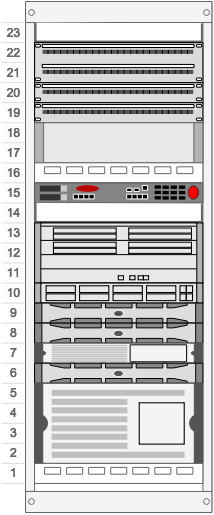
\includegraphics[]{fig2}
	\caption{Exemplo de figura sem escala}
	\label{fig2}
\end{figure}

Você pode rotacionar figuras também. Para isso utilize o parâmetro angle=-90. Repare que a escala da figura foi modificada pelo parametro height. Você também pode utilizar scale

\begin{figure}
	\centering
	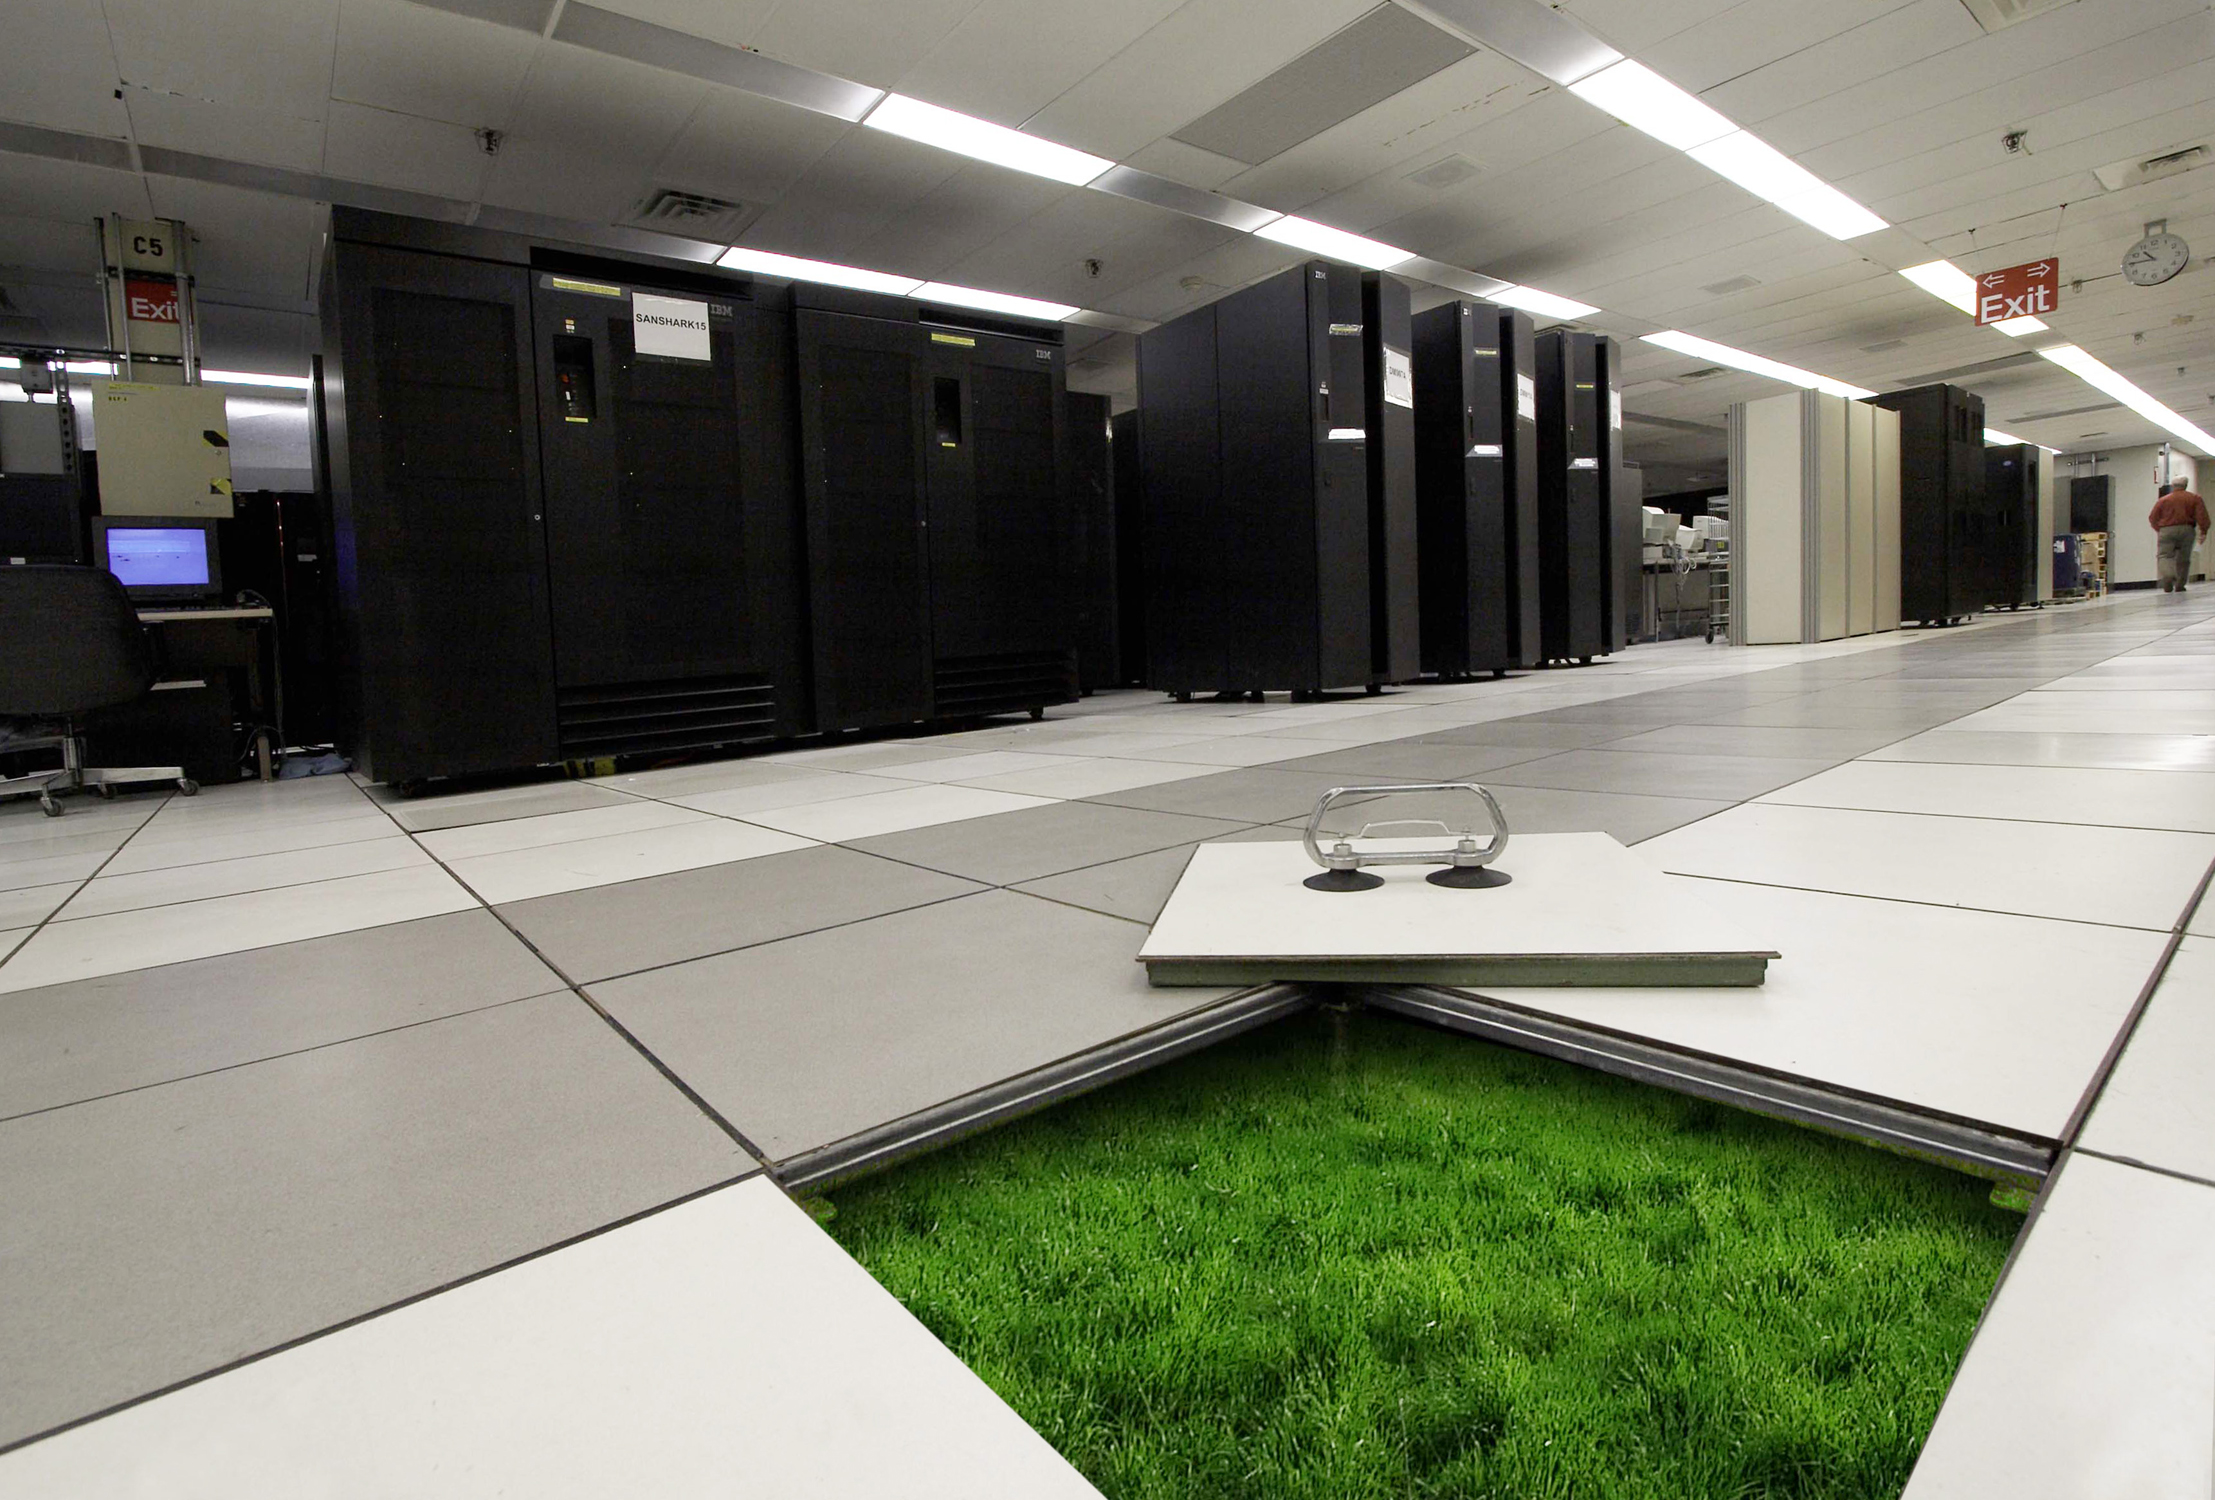
\includegraphics[height=\textwidth,angle=-90]{fig3}
	\caption{Exemplo de figura rotacionada}
	\label{fig3}
\end{figure}




%% ***********************************************************************
%% === ate aqui    =====  ================================================
%% ***********************************************************************

\end{document}